\documentclass[12pt]{article}

%----------------------------------------------------------------------------------------
%	PACKAGES
%----------------------------------------------------------------------------------------

\usepackage{cite}
\usepackage{graphicx}
\usepackage{caption}
\usepackage{subcaption}
\usepackage{amssymb}
\usepackage{mathtools}
\usepackage{amsmath}
\usepackage{isomath}
\usepackage{hyperref}
\usepackage[hypcap]{caption}
\usepackage{listings}
\usepackage{color}
\usepackage{cleveref}

%----------------------------------------------------------------------------------------
%	PAGE & LINKS SETUP
%----------------------------------------------------------------------------------------

% Default margins are too wide all the way around. I reset them here
\setlength{\topmargin}{-.5in}
\setlength{\textheight}{9in}
\setlength{\oddsidemargin}{.125in}
\setlength{\textwidth}{6.25in}

% Graphics folder path
\graphicspath{ {./images/} }

% Hyperlinks and URL setup
\hypersetup{
    bookmarks=true, % show bookmarks bar?
    unicode=false, % non-Latin characters in Acrobat’s bookmarks
    pdftoolbar=true, % show Acrobat’s toolbar?
    pdfmenubar=true, % show Acrobat’s menu?
    pdffitwindow=false, % window fit to page when opened
    pdfstartview={FitH}, % fits the width of the page to the window
    pdftitle={IDAPI Coursework 4}, % title
    pdfauthor={Hesam Ipakchi, Yijie Ge}, % author
    pdfsubject={IDAPI Coursework 4}, % subject of the document
    pdfcreator={Hesam Ipakchi}, % creator of the document
    pdfproducer={Hesam Ipakchi, Yijie Ge}, % producer of the document
    pdfkeywords={Hesam Ipakchi, Yijie Ge, IDAPI Coursework 4}, % list of keywords
    pdfnewwindow=true, % links in new window
    colorlinks=true, % false: boxed links; true: colored links
    linkcolor=red, % color of internal links (change box color with linkbordercolor)
    citecolor=blue, % color of links to bibliography
    filecolor=black, % color of file links
    urlcolor=black  % color of external links
}
\urlstyle{same}

% Subreferences Setup
\captionsetup{subrefformat=parens}

%----------------------------------------------------------------------------------------
%	DEFINITIONS OF NEW COMMANDS
%----------------------------------------------------------------------------------------


%----------------------------------------------------------------------------------------
%	BEGIN DOCUMENT
%----------------------------------------------------------------------------------------

\begin{document}

% Consider all references (including those not cited) for biliography
\nocite{*}

%----------------------------------------------------------------------------------------
%	TITLE PAGE
%----------------------------------------------------------------------------------------

\title{\textbf{Intelligent Data Analysis and Probabilistic Inference Coursework 4}}
\author{Hesam Ipakchi (00648378), Yijie Ge (00650073), Joysen Goes (00649883)\\Imperial College London}
\date{\today}
% make title page without page number in footer
\clearpage\maketitle
\thispagestyle{empty}

%----------------------------------------------------------------------------------------
%	RESULTS
%----------------------------------------------------------------------------------------

\newpage
\thispagestyle{plain}
\mbox{}

% start page numbers arabic style (1,2,3...)
\pagenumbering{arabic} 

\section {IDAPIResults04.txt File Contents}
\label{sec:resultsFileContents}

\lstinputlisting[breaklines=true]{IDAPIResults04.txt}

%----------------------------------------------------------------------------------------
%	Task 4.3 Eigenfaces
%----------------------------------------------------------------------------------------

\newpage
\thispagestyle{plain}
\mbox{}

\section {Task 4.3 Eigenfaces}
\label{sec:task4.3Eigenfaces}

\cref{fig:task4.3Eigenfaces} shows the eigenface images we created in task 4.3. There are 10 of them, numbered from 0 to 9, since there were 10 principal components given.

\begin{figure}
	\centering
	\begin{subfigure}[b]{0.20\textwidth}
		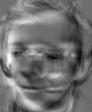
\includegraphics[width=\textwidth]{Task4.3_Images/PrincipalComponent0.jpg}
		\caption{Eigenface: 0}
	\end{subfigure}\quad
	\begin{subfigure}[b]{0.20\textwidth}
		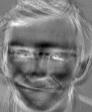
\includegraphics[width=\textwidth]{Task4.3_Images/PrincipalComponent1.jpg}
		\caption{Eigenface: 1}
	\end{subfigure}\quad
	\begin{subfigure}[b]{0.20\textwidth}
		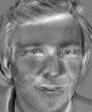
\includegraphics[width=\textwidth]{Task4.3_Images/PrincipalComponent2.jpg}
		\caption{Eigenface: 2}
	\end{subfigure}\quad
	\begin{subfigure}[b]{0.20\textwidth}
		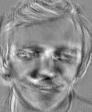
\includegraphics[width=\textwidth]{Task4.3_Images/PrincipalComponent3.jpg}
		\caption{Eigenface: 3}
	\end{subfigure}\\
	\begin{subfigure}[b]{0.20\textwidth}
		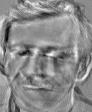
\includegraphics[width=\textwidth]{Task4.3_Images/PrincipalComponent4.jpg}
		\caption{Eigenface: 4}
	\end{subfigure}\quad
	\begin{subfigure}[b]{0.20\textwidth}
		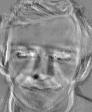
\includegraphics[width=\textwidth]{Task4.3_Images/PrincipalComponent5.jpg}
		\caption{Eigenface: 5}
	\end{subfigure}\quad
	\begin{subfigure}[b]{0.20\textwidth}
		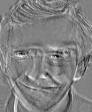
\includegraphics[width=\textwidth]{Task4.3_Images/PrincipalComponent6.jpg}
		\caption{Eigenface: 6}
	\end{subfigure}\quad
	\begin{subfigure}[b]{0.20\textwidth}
		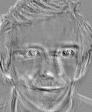
\includegraphics[width=\textwidth]{Task4.3_Images/PrincipalComponent7.jpg}
		\caption{Eigenface: 7}
	\end{subfigure}\\
	\begin{subfigure}[b]{0.20\textwidth}
		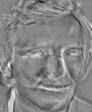
\includegraphics[width=\textwidth]{Task4.3_Images/PrincipalComponent8.jpg}
		\caption{Eigenface: 8}
	\end{subfigure}\quad
	\begin{subfigure}[b]{0.20\textwidth}
		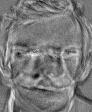
\includegraphics[width=\textwidth]{Task4.3_Images/PrincipalComponent9.jpg}
		\caption{Eigenface: 9}
	\end{subfigure}\quad
	\caption[Plots of eigenface images created in task 4.3]{\label{fig:task4.3Eigenfaces} The eigenface images created in task 4.3}
\end{figure}

%----------------------------------------------------------------------------------------
%	Task 4.4 Partial Reconstructions
%----------------------------------------------------------------------------------------

\newpage
\thispagestyle{plain}
\mbox{}

\section {Task 4.4 Partial Reconstructions}
\label{sec:task4.4PartialReconstructions}

\cref{fig:task4.4ReconstructedImages} shows the partial reconstructions of image c.pgm created in task 4.4. The first image (Reconstructed Image: 0) represents the mean image, whilst the $i-th$ image (Reconstructed Image: $i$) represents the mean image plus all up to $i-th$ principal component. There are 11 images in the figure since there are 10 principal components (including the one associated with a zero eigenvalue).

\begin{figure}
	\centering
	\begin{subfigure}[b]{0.20\textwidth}
		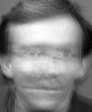
\includegraphics[width=\textwidth]{Task4.3_Images/ReconstructedImage0.jpg}
		\caption{Reconstructed Image: 0}
	\end{subfigure}\quad
	\begin{subfigure}[b]{0.20\textwidth}
		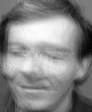
\includegraphics[width=\textwidth]{Task4.3_Images/ReconstructedImage1.jpg}
		\caption{Reconstructed Image: 1}
	\end{subfigure}\quad
	\begin{subfigure}[b]{0.20\textwidth}
		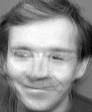
\includegraphics[width=\textwidth]{Task4.3_Images/ReconstructedImage2.jpg}
		\caption{Reconstructed Image: 2}
	\end{subfigure}\quad
	\begin{subfigure}[b]{0.20\textwidth}
		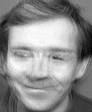
\includegraphics[width=\textwidth]{Task4.3_Images/ReconstructedImage3.jpg}
		\caption{Reconstructed Image: 3}
	\end{subfigure}\\
	\begin{subfigure}[b]{0.20\textwidth}
		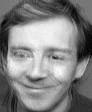
\includegraphics[width=\textwidth]{Task4.3_Images/ReconstructedImage4.jpg}
		\caption{Reconstructed Image: 4}
	\end{subfigure}\quad
	\begin{subfigure}[b]{0.20\textwidth}
		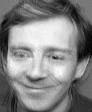
\includegraphics[width=\textwidth]{Task4.3_Images/ReconstructedImage5.jpg}
		\caption{Reconstructed Image: 5}
	\end{subfigure}\quad
	\begin{subfigure}[b]{0.20\textwidth}
		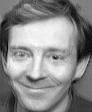
\includegraphics[width=\textwidth]{Task4.3_Images/ReconstructedImage6.jpg}
		\caption{Reconstructed Image: 6}
	\end{subfigure}\quad
	\begin{subfigure}[b]{0.20\textwidth}
		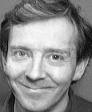
\includegraphics[width=\textwidth]{Task4.3_Images/ReconstructedImage7.jpg}
		\caption{Reconstructed Image: 7}
	\end{subfigure}\\
	\begin{subfigure}[b]{0.20\textwidth}
		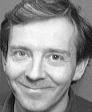
\includegraphics[width=\textwidth]{Task4.3_Images/ReconstructedImage8.jpg}
		\caption{Reconstructed Image: 8}
	\end{subfigure}\quad
	\begin{subfigure}[b]{0.20\textwidth}
		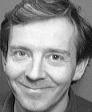
\includegraphics[width=\textwidth]{Task4.3_Images/ReconstructedImage9.jpg}
		\caption{Reconstructed Image: 9}
	\end{subfigure}\quad
\begin{subfigure}[b]{0.20\textwidth}
		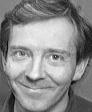
\includegraphics[width=\textwidth]{Task4.3_Images/ReconstructedImage10.jpg}
		\caption{Reconstructed Image: 10}
	\end{subfigure}\quad
	\caption[Plots of partial reconstructions of image c.pgm in task 4.4]{\label{fig:task4.4ReconstructedImages} Partial reconstructions of image c.pgm in task 4.4}
\end{figure}

%----------------------------------------------------------------------------------------
%	Task 4.6 Eigenfaces
%----------------------------------------------------------------------------------------

\newpage
\thispagestyle{plain}
\mbox{}

\section {Task 4.6 Eigenfaces}
\label{sec:task4.6Eigenfaces}

\cref{fig:task4.6Eigenfaces} shows the eigenface images we created in task 4.6. The figure comprises of 5 images, numbered from 0 to 4, since we plotted only principal components with non-zero eigenvalues (6 principal components existed in total as there were 6 images labelled from a to f, but one had a zero eigenvalue). Note that for partial reconstruction, we did not need to consider the principal component with zero eigenvalue, thus we did not plot the eigenface associated with the zero eigenvalue in this figure.

\begin{figure}
	\centering
	\begin{subfigure}[b]{0.20\textwidth}
		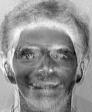
\includegraphics[width=\textwidth]{Task4.6_Images/PrincipalComponent0.jpg}
		\caption{Eigenface: 0}
	\end{subfigure}\quad
	\begin{subfigure}[b]{0.20\textwidth}
		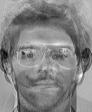
\includegraphics[width=\textwidth]{Task4.6_Images/PrincipalComponent1.jpg}
		\caption{Eigenface: 1}
	\end{subfigure}\quad
	\begin{subfigure}[b]{0.20\textwidth}
		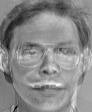
\includegraphics[width=\textwidth]{Task4.6_Images/PrincipalComponent2.jpg}
		\caption{Eigenface: 2}
	\end{subfigure}\\
	\begin{subfigure}[b]{0.20\textwidth}
		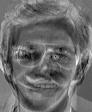
\includegraphics[width=\textwidth]{Task4.6_Images/PrincipalComponent3.jpg}
		\caption{Eigenface: 3}
	\end{subfigure}\quad
	\begin{subfigure}[b]{0.20\textwidth}
		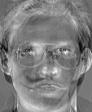
\includegraphics[width=\textwidth]{Task4.6_Images/PrincipalComponent4.jpg}
		\caption{Eigenface: 4}
	\end{subfigure}\quad
	\caption[Plots of eigenface images created in task 4.6]{\label{fig:task4.6Eigenfaces} The eigenface images created in task 4.6}
\end{figure}

%----------------------------------------------------------------------------------------
%	Task 4.6 Partial Reconstructions
%----------------------------------------------------------------------------------------

\newpage
\thispagestyle{plain}
\mbox{}

\section {Task 4.6 Partial Reconstructions}
\label{sec:task4.6PartialReconstructions}

\cref{fig:task4.6ReconstructedImages} shows the partial reconstructions of image c.pgm created in task 4.6. The first image (Reconstructed Image: 0) represents the mean image, whilst the $i-th$ image (Reconstructed Image: $i$) represents the mean image plus all up to $i-th$ principal component. There are 6 images in the figure since there are 5 principal components with non-zero eigenvalues.

\begin{figure}
	\centering
	\begin{subfigure}[b]{0.20\textwidth}
		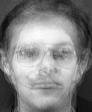
\includegraphics[width=\textwidth]{Task4.6_Images/ReconstructedImage0.jpg}
		\caption{Reconstructed Image: 0}
	\end{subfigure}\quad
	\begin{subfigure}[b]{0.20\textwidth}
		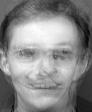
\includegraphics[width=\textwidth]{Task4.6_Images/ReconstructedImage1.jpg}
		\caption{Reconstructed Image: 1}
	\end{subfigure}\quad
	\begin{subfigure}[b]{0.20\textwidth}
		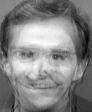
\includegraphics[width=\textwidth]{Task4.6_Images/ReconstructedImage2.jpg}
		\caption{Reconstructed Image: 2}
	\end{subfigure}\\
	\begin{subfigure}[b]{0.20\textwidth}
		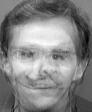
\includegraphics[width=\textwidth]{Task4.6_Images/ReconstructedImage3.jpg}
		\caption{Reconstructed Image: 3}
	\end{subfigure}\quad
	\begin{subfigure}[b]{0.20\textwidth}
		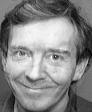
\includegraphics[width=\textwidth]{Task4.6_Images/ReconstructedImage4.jpg}
		\caption{Reconstructed Image: 4}
	\end{subfigure}\quad
	\begin{subfigure}[b]{0.20\textwidth}
		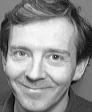
\includegraphics[width=\textwidth]{Task4.6_Images/ReconstructedImage5.jpg}
		\caption{Reconstructed Image: 5}
	\end{subfigure}\quad
	\caption[Plots of partial reconstructions of image c.pgm in task 4.6]{\label{fig:task4.6ReconstructedImages} Partial reconstructions of image c.pgm in task 4.6}
\end{figure}


\end{document}